\subsection{Support to DUDES composition}
\label{sec:parsing-support-dudes-composition}

In this section we show how our parser supports DUDES composition though \textit{main variable mappings}.
%
First of all, we state here some useful definitions.
%
An \textit{obfuscated variable} is a main variable of a DUDES that is lost at time $t_{1}$ due to substitution, though it should be referenced by some other DUDES at time $t_{2}>t_{1}$.
%
We call \textit{obfuscating substitution} a DUDES substitution that creates an obfuscating variable.

In Figure~\ref{fig:obfuscating-substitution-1} we show an example of obfuscating substitution. 
%
Let us consider the question \textit{'did Microsoft acquire an italian company?'}.
%
We have the main LTAG/DUDES (a), the waiting LTAG/DUDES (b) and the ambiguous LTAG/DUDES (c).
%
The substitution of (b) in (a) is an obfuscating substitution, because once executed, the resulting main LTAG/DUDES in Figure~\ref{fig:obfuscating-substitution-2}.
%
Notice that the resulting main LTAG/DUDES does not have the main variable any more, due to the normal DUDES substitution.
%
Such a situation makes the adjunction of (c) loose its semantic value, due to the absence of the main variable.

Our parser overcome this limitation by detecting obfuscating substitutions. 
%
In particular, it records obfuscated variable, making them accessible by successive adjunctions.
%
In this way, the semantic value of (c) would have never been lost.
%
When (c) is processed, the parser detects that it is looking for an obfuscated variable and makes it temporaly available in the semantics of the main LTAG/DUDES.
%
Once the obfuscated variable have been used, it will never be considered any more.

\begin{figure}[tp]
	\caption{An example of obfuscating substitution (a),(b),(c).}
	\label{fig:obfuscating-substitution-1}
	\begin{tabular}{ p{10em} p{10em} p{10em} }
		\begin{center}
		(a)
		\begin{tikzpicture}
			\Tree [.S [.V did ] [.S [.DP  Microsoft ] [.VP [.V acquire ] [.DP [.DET an ] [.NP$\downarrow$ ] ] ] ] ]
		\end{tikzpicture}
		\end{center}		
		&
		\begin{center}
		(b)
		\begin{tikzpicture}
			\Tree [.NP company ]	
		\end{tikzpicture}
		\end{center}		
		&
		\begin{center}
		(c)
		\begin{tikzpicture}
			\Tree [.NP [.ADJ italian ] [.NP* ] ]
		\end{tikzpicture}
		\end{center}		
		
		\\
			
		\begin{center}
		\begin{tabular}{|c|l|}
		\hline
		\mbox{} & x y \\ 
		\hline
		\multicolumn{2}{|l|}{
			$isAcquiredBy(x,y)$
		}\\
		\multicolumn{2}{|l|}{
			$y=Microsoft$
		}\\
		\hline
		\multicolumn{2}{|l|}{
			\mbox{$(x,NP)$}
		} \\
		\hline
		\end{tabular}
		\end{center}
		&
		\begin{center}
		\begin{tabular}{|c|l|}
		\hline
		\mbox{x} & x \\ 
		\hline
		\multicolumn{2}{|l|}{
			$Company(x)$
		}\\
		\hline
		\multicolumn{2}{|l|}{
			\mbox{}
		} \\
		\hline
		\end{tabular}
		\end{center}	
		&
		\begin{center}
		\begin{tabular}{|c|l|}
		\hline
		\mbox{x} & x y \\ 
		\hline
		\multicolumn{2}{|l|}{
			$hasHeadquarter(x,y)$
		}\\
		\multicolumn{2}{|l|}{
			$y=Italy$
		}\\
		\hline
		\multicolumn{2}{|l|}{
			\mbox{}
		} \\
		\hline
		\end{tabular}
		\end{center}
	\end{tabular}
\end{figure}

\begin{figure}[tp]
	\caption{An example of obfuscating substitution. The substitution obfuscates the main variable.}
	\label{fig:obfuscating-substitution-2}
	\begin{tabular}{ p{10em} p{10em} }
		\begin{center}
		\begin{tikzpicture}
		\Tree [.S [.V did ] [.S [.DP  Microsoft ] [.VP [.V acquire ] [.DP [.DET an ] [.NP company ] ] ] ] ]
		\end{tikzpicture}
		\end{center}
		\begin{center}
		\begin{tabular}{|c|l|}
			\hline
			\mbox{} & x y \\ 
			\hline
			\multicolumn{2}{|l|}{
				$isAcquiredBy(x,y)$
			}\\
			\multicolumn{2}{|l|}{
				$y=Microsoft$
			}\\	
			\multicolumn{2}{|l|}{
				$Company(x)$
			}\\			
			\hline
			\multicolumn{2}{|l|}{
				\mbox{}
			} \\
			\hline
		\end{tabular}
		\end{center}	
	\end{tabular}
\end{figure}

\begin{figure}[tp]
	\caption{An example of obfuscating substitution. The obfuscated variable is not accessible for the adjunction, causing the main variabl refence to be lost.}
	\label{fig:obfuscating-substitution-3}
	\begin{tabular}{ p{10em} }
		\begin{center}
		\begin{tikzpicture}
			\Tree [.S [.V did ] [.S [.DP  Microsoft ] [.VP [.V acquire ] [.DP [.DET an ] [.NP [.ADJ italian ] company ] ] ] ] ]
		\end{tikzpicture}
		\end{center}	
		\\
		\begin{center}
			\begin{tabular}{|c|l|}
				\hline
				\mbox{} & x y z\\ 
				\hline
				\multicolumn{2}{|l|}{
					$isAcquiredBy(x,y)$
				}\\
				\multicolumn{2}{|l|}{
					$y=Microsoft$
				}\\
				\multicolumn{2}{|l|}{
					$Company(x)$
				}\\
				\multicolumn{2}{|l|}{
					$hasHeadquarter(z,t)$
				}\\
				\multicolumn{2}{|l|}{
					$t=Italy$
				}\\
				\hline
				\multicolumn{2}{|l|}{
					\mbox{}
				} \\
				\hline
			\end{tabular}
		\end{center}	
	\end{tabular}
\end{figure}
